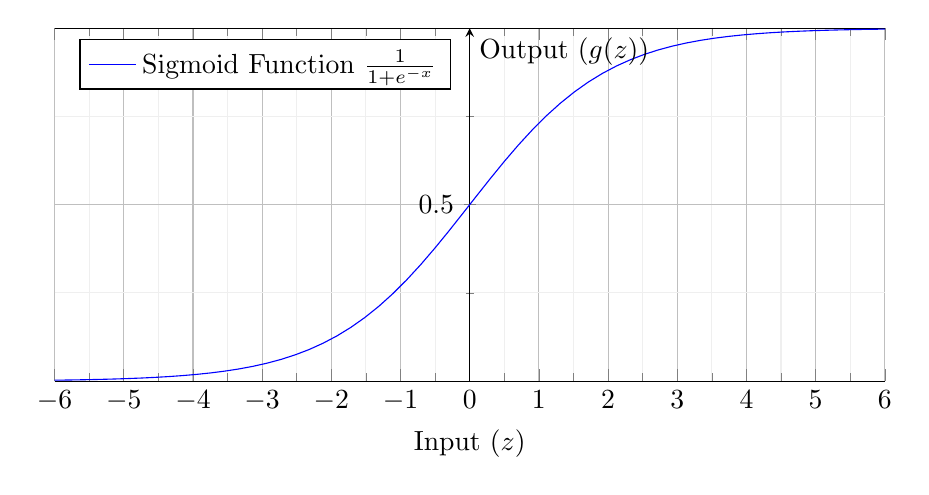
\begin{tikzpicture}
    \begin{axis}[
        xmin = -6, xmax = 6,
        ymin = 0, ymax = 1,
        width = \textwidth,
        height = 0.5\textwidth,
        xtick distance = 1,
        ytick distance = 1,
        grid = both,
        minor tick num = 1,
        major grid style = {lightgray},
        minor grid style = {lightgray!25},
        xlabel = {Input ($z$)},
        ylabel = {Output ($g(z)$)},
        legend cell align = {left},
        legend pos = north west,
        ytick={0,.5,1},
        axis y line=middle
    ]
     
    \addplot%
    [
        blue,%
        mark=none,
        samples=100,
        domain=-10:10,
    ]
    (x,{1/(1+exp(-x))});      
     
    % Add legend
    \addlegendentry{Sigmoid Function $\frac{1}{1 + e^{-x}}$}
     
    \end{axis}
    \end{tikzpicture}